#should come under Optimization chapter intenals

\section{UpdaterClass}
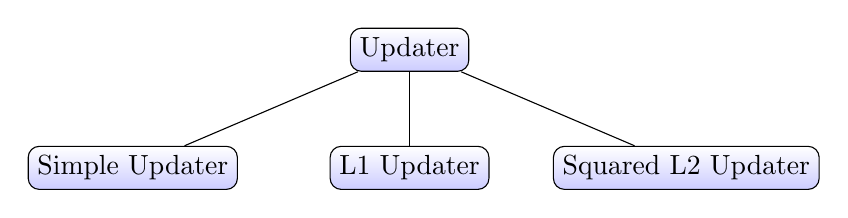
\begin{tikzpicture}[sibling distance=10em,
  every node/.style = {shape=rectangle, rounded corners,
    draw, align=center,
    top color=white, bottom color=blue!20}]]
  \node {Updater}
     child { node {Simple Updater} }
     child { node {L1 Updater} }
     child { node {Squared L2 Updater} };
\end{tikzpicture}


\section{Simple Updater}
Eg Case:
stepSize = 1
Number of iteration = 100

thisIterStepSize = stepSize / math.sqrt(iter)

iter         thisIterStepSize
1             1 / 1      = 1
2             1 / 1.414  = 0.707
3             1 / 1.732  = 0.577
4             1 / 2      = 0.5
.
.
.
100           1 / 10    = 0.1

y += x * a
          a                   x               y
brzAxpy(-thisIterStepSize, gradient.toBreeze, brzWeights)


\section{L1 Updater or Lasso Regression}


\section{Squared L2 Updater or Rigid Regression}
    // w' = w - thisIterStepSize * (gradient + regParam * w)
    // w' = w - thisIterStepSize * gradient - thisIterStepSize * regParam * w
    // w' = w - thisIterStepSize * regParam * w - thisIterStepSize * gradient
    // w' = (1 - thisIterStepSize * regParam) * w - thisIterStepSize * gradient

